\documentclass{article}


\usepackage{array}
\usepackage{etoolbox}
\usepackage{fancyhdr}
\usepackage{geometry} 
\usepackage{graphicx}
\usepackage{lastpage}
\usepackage{soul}
\usepackage{titling}
\usepackage{subcaption}

%%%%%%%%%%%%%%%%%%%%%%%%%%%%%%%%%%%%%%%%%%%%%%%%%%%%%%%%%%%%
% BEGIN METADATA: Edit the following as appropriate
%%%%%%%%%%%%%%%%%%%%%%%%%%%%%%%%%%%%%%%%%%%%%%%%%%%%%%%%%%%%

\title{Mycelium Network Optimization In The Context Of Karachi's Networks}  % the title of your project
\newcommand\shorttitle{\thetitle}  % if needed: a shorter title for the document header
% Team members.
\newcommand\firstname{Syed Ammar Mahdi}  % full name
\newcommand\firstid{sm03691}         % ID, e.g. xy01234
\newcommand\secondname{Bahzad Ahmed Badvi} % full name
\newcommand\secondid{bb05083}        % ID, e.g. xy01234
\newcommand\thirdname{Ramis Raza}  % full name
\newcommand\thirdid{rr05253}         % ID, e.g. xy01234
\newcommand\fourthname{Maaz Saeed}  % full name
\newcommand\fourthid{ms05050}         % ID, e.g. xy01234
\newcommand\fifthname{Syeda Zainab Fatima}  % full name
\newcommand\fifthid{sf05166}         % ID, e.g. xy01234

%%%%%%%%%%%%%%%%%%%%%%%%%%%%%%%%%%%%%%%%%%%%%%%%%%%%%%%%%%%%
% END METADATA: Do not edit the preamble any further.
%%%%%%%%%%%%%%%%%%%%%%%%%%%%%%%%%%%%%%%%%%%%%%%%%%%%%%%%%%%%

\pagestyle{fancy}
\lhead{Kaavish Proposal}
\chead{\shorttitle}
\rhead{Fall 2021}
\cfoot{Page \thepage}
\renewcommand{\footrulewidth}{0.4pt}

\newcommand\instruction[1]{\textit{#1}}

\begin{document}

% Cover page.
\begin{titlepage}

\center % Center everything on the page
 
%----------------------------------------------------------------------------------------
%	HEADING SECTIONS
%----------------------------------------------------------------------------------------

\textsc{
  {\LARGE \bf \thetitle}\\\bigskip\bigskip % Your Project Title
  {\large
    Kaavish Project Proposal\\\bigskip
    By}}\\\bigskip 

%----------------------------------------------------------------------------------------
%	AUTHOR SECTION
%----------------------------------------------------------------------------------------

{\large
  \begin{tabular}{ll}
    \firstname & (\firstid@st.habib.edu.pk) \\
    \secondname & (\secondid@st.habib.edu.pk) \\
    \thirdname & (\thirdid@st.habib.edu.pk) \\
    \ifdef{\fourthname}{\fourthname & (\fourthid@st.habib.edu.pk) \\}{}
    \ifdef{\fifthname}{\fifthname & (\fifthid@st.habib.edu.pk) \\}{}
  \end{tabular}
}
\bigskip\bigskip\bigskip

{\large \today}\\\bigskip\bigskip


\includegraphics[height=5cm]{HU_logo_new.png}\\\bigskip
 
%----------------------------------------------------------------------------------------
{\large
  In partial fulfillment of the requirement for \\\medskip
Bachelor of Science \\\medskip
Computer Science
}\\\bigskip\bigskip\bigskip

{\large
  \textsc{
    Dhanani School of Science and Engineering\\\bigskip
    Habib University\\\bigskip 
    Fall 2021
  }\\\bigskip\bigskip 
  Copyright @ 2021 Habib University
}

\end{titlepage}


%%%%%%%%%%%%%%%%%%%%%%%%%%%%%%%%%%%%%%%%%%%%%%%%%%%%%%%%%%%%
% DATA: Populate the rest of the document as instructed.
%%%%%%%%%%%%%%%%%%%%%%%%%%%%%%%%%%%%%%%%%%%%%%%%%%%%%%%%%%%%

\section{Problem definition}
%\instruction{Describe the problem that the project addresses.}

Ever since \textit{physarum polycephalum}, a.k.a "the Yellow slime mould", started being studied for its computational intelligence, it has garnered a great deal of attention in the world of biology-inspired computing with respects to network science, logic, path-finding, and many other applications in computing. This is due to the changing topology of the mycelial network as it explores its environment and searches for food, displaying many intelligent behaviors in the process. Sun has stated this intelligence can be exploited to solve various network optimization problems. Amongst other findings, experiments related to the slime mould confirm that it can optimize networks, solve mazes and generate a minimum spanning graph with use of its foraging mechanics \cite{10.2307/40508592} \cite{article}.

By 2018, a new research was published where Adamatzky proposed that Fungi Basidiomycetes are a better candidate for such experimentation than \textit{physarum polycephalum} \cite{doi:10.1098/rsfs.2018.0029} . This is due to the fact that the former is less susceptible to environmental factors, is easier to obtain and manipulate. He proposed that since both are analogous to each other, experiments done on \textit{physarum polycephalum} can be replicated using Mycelium networks from Fungi Basidiomycetes.

We aim to fill this space in the field of Bio-inspired computing by replicating with Mycelium networks, the Tokyo Rail Network experiment which was performed using \textit{physarum polycephalum} \cite{10.2307/40508592}. With the obtained results, we aim to produce an algorithm to mimic the foraging and growth pattern of Mycelium networks.

\section{Social relevance}

Ease of access to transport is one of the most important problem any big city has to solve. Unfortunately, Karachi - one of the most populated cities in the world - does not have a mass transit system. Previous attempts to solve this problem have failed for several reasons, such as development-related issues, political turmoil, and sub-optimal design.

By using mycelium to map Karachi's transport network, we provide an alternate to the currently existing transport network routes. This is similar to the experiment done using \textit{physarum polycephalum} to re-map Tokyo's subway networks. The result of the Tokyo experiment was that the slime mould managed to optimize Tokyo's subway better than humans designed it \cite{sun2019physaruminspired}.

By repeating the experiment with mycelium of\textit{pleurotus ostreatus} in the context of Karachi's networks, we hope to provide a roadmap to solving some of the most pressing issues in the city, including transport and possibly sewage flow.

\section{Originality/Novelty}


\textit{Physarum polycephalum} has been used for many years in solving the travelling Salesman problem. However, in recent years, \textit{physarum polycephaum} have been replaced with fungal mycelium of the genus \textit{Basidiomycetes} as a viable replacement. Although Adamatzky claims that mycelium of \textit{pleurotus ostreatus},  (a.k.a the "Oyster mushroom"), is phenomenologically similar to the slime mould \textit{physarum polycephalum} \cite{doi:10.1098/rsfs.2018.0029}, there has been no extensive research to back this claim as of yet. Our approach, therefore, is novel as it is the first time mycelium is being used to solve the same network optimization problems that have been previously solved using slime moulds for several years, including the Steiner tree and shortest path problems \cite{sun2019physaruminspired}.

There have also been mathematical and computational models of physarum developed before, such as the one that mathematically confirms that physarum can solve the shortest path problem \cite{Bonifaci_2012}. A similar model for mycelium has yet to be seen in the literature.

Finally, problem of a large city's transport network has previously been solved both for the road networks of Tokyo \cite{10.2307/40508592} and USA \cite{Adamatzky2016} using slime mould. The experiment has not yet been replicated with mycelium; doing so would confirm whether or not mycelium has the same computational intelligence as physarum. This approach would also apply use mycelium to optimize the transport networks of Karachi, which has previously not been studied using bio-inspired networking approaches.

\section{CS contribution}


Path optimization is an extensively studied field of graph theory. In problems that involve optimization, it is often useful to find a minimum spanning tree (MST) of a weighted graph. To minimize the cost of certain variables, algorithms are often used to gradually build a spanning tree (or many such trees) as intermediate steps in the process of finding the minimum spanning tree. In many such problems involving combinatorial optimization, exhaustive search does not serve as a viable solution with large data-sets \cite{5368915}. However, it functions as per the domain of those optimization problems in which the set of constructive solutions is discrete or can be reduced to discrete, and in which the goal is to find the best solution. The best solutions are, however, limited by the tricky math problems that sit at the center of these optimization problems. Typical problems are the traveling salesman problem ("TSP"), the minimum spanning tree problem ("MST"), and the knapsack problem. These are complex algorithmic problems to solve when faced with a large data set. The current workable solutions for such problems are based on “heuristics” to provide exact solutions for some versions of these problems \cite{Ogheneovo2016AHG}. For the case of TSP i.e. an NP-hard problem, the existing researches on Physarum-inspired algorithms (PAs) are proved to challenge some widely used evolutionary algorithms such as the ant colony optimization algorithm, the genetic algorithm, and the particle swarm optimization algorithm for real-world large instances \cite{10.1007/978-3-319-11857-4_20}. However, the existing researches on PAs are still immature and far from being fully recognized. By replicating experiments using Mycelium networks, the aim is to analyze the network optimization problems and applications that have been challenged by PAs using Mycelium-inspired networking models. These models will be devised by mathematically representing the behaviour of Mycelium networks using evolutionary algorithms. The project further aims to generalise a successful simulating model for any network according to its topology and real-world applications.

\section{Scope and Deliverables}


\begin{itemize}
    \item Scope: The project is an inter-disciplinary one involving both Computer Science and Microbiology. As such, we feel that a team of four members is justified to have two individuals working on the biology lab work and another two working on the algorithm design and simulation programming part.
    
    We shall rotate team members where necessary between the two roles not only to avoid stagnation, but also to ensure that each member can make a contribution to all parts of the project rather than just focusing on one aspect.
    \item Deliverables: The approach for our deliverables will be largely adapted from following the procedure for unraveling slime mould intelligence as outlined by Sun \cite{sun2019physaruminspired}.
    
    \begin{enumerate}
        \item Perform experiments revealing mycelium intelligence on agar.
        \item Based on the experimental results, model the mycelium intelligence (algorithm design, heuristic methods, agent-based modelling, etc).
        \item Customize the model for our applications and develop front-end software for running the simulation of our model.
    \end{enumerate}
    
    Note that the approach outlined was for physarum-inspired networking models, but is generalizable to mycelium networks as well.
    
    The following SMART deliverables have been identified by our team:
    
    \begin{itemize}
        \item \textbf{A model of mycelium growth in a generalised environment:} The model will be based on the real behaviour of mycelium as it colonizes an agar plate in search of food. Algorithms, heuristic approach and agent-based models can all potentially be used in this model.
        \item \textbf{Front-end simulation application using the simulation over transport networks for Karachi:} The simulation should have several parameters that can be adjusted, including addition of nodes, changing terrain, and changing environmental conditions. An option for switching between slime mould and oyster mushroom mycelium may also be included in the simulation, to compare and contrast the behaviour of both organisms.
        \item \textbf{Viable mycelium cultures for experimentation in the lab:} Multiple strains will be obtained from grain spawn colonized on agar. From the isolated strains, the ones showing rapid growth, resistance to contamination and temperature fluctuations will be selected. The experiment will be repeated with several mycelium strains for accuracy of results.
        \item A 3D-printed, scaled down model of Karachi's map on an agar plate. This will be the model used for colonization and studying network optimization, as was done in previous experiments \cite{10.2307/40508592} \cite{Adamatzky2016}
        
    \end{itemize}
\end{itemize}

\section{Feasibility}


The simulation part of the project can be done on any modern computer with sufficient computing power. Simulation models can be trained in Java using OR-Tools i.e. an open source software suite for optimization, tuned for tackling the world's toughest problems in vehicle routing, flows, integer and linear programming, and constraint programming. The biology lab experiments, on the other hand, requires some more specialized hardware. Fortunately, the Habib University laboratories are already equipped with everything needed to perform these experiments.

A live culture of \textit{physarum polycephalum} is both difficult to acquire and work with in Pakistan. The slime mould is native to cooler countries and will not thrive well in the hot climate of Karachi. It is also more difficult to manipulate and work with in the laboratory.

\textit{Pleurotus ostreatus}, on the other hand, is very easy to acquire in Pakistan as many local mushroom farms supply it. This organism is also the species recommended by Adamztky and others (citation needed) due to being much easier to manipulate and work with in the lab. The spawn can be acquired locally from different vendors for a low cost. Once the spawn is acquired, grains can be placed on agar or cardboard to create viable cultures of \textit{pleurotus ostreatus} mycelium. The different mycelium strains from the spawn will be further selected and isolated to produce genetic traits conducive to experimentation.

Live culture work can be performed in front of a laminar flow hood, as is the standard in lab mycology. A flow hood can be constructed either at home or sourced from a local vendor, although at a relatively high cost. In the absence of a flow hood, a still air box can be substituted to work with the cultures. Both SABs and flow hoods drastically lower the possibility of culture contamination from live mould spores, bacteria and other micro-organisms suspended in air. The working of both devices can be explained, but is beyond the scope of this document.

\section{Team dynamics}

Each team member is listed along with their respective strengths and weaknesses below:
\begin{itemize}
    \item Syed Ammar Mahdi
    \begin{enumerate}
        \item \textbf{Relevant courses:}
        \begin{enumerate}
            \item Algorithms: Design \& Analysis
            \item Data Structures and Algorithms
            \item Discrete Math
            \item Energy/Energy Lab
            \item Networks, Games, and Collective Behaviour
        \end{enumerate}
        \item \textbf{Relevant Technical Strengths:}
        \begin{enumerate}
            \item Experience growing mycelium cultures
            \item Experience with working with agar, microbiology lab work
            \item Technical knowledge of how to transfer these skills to other team members
            \item Good working knowledge of network science and graph theory
        \end{enumerate}
        \item \textbf{Relevant Technical Weaknesses:}
        \begin{enumerate}
            \item Lackluster coding skills
            \item Average at advanced mathematics
        \end{enumerate}
    \end{enumerate}
    \item Bahzad Ahmed Badvi
    \begin{enumerate}
        \item \textbf{Relevant courses:}
        \begin{enumerate}
            \item Algorithms: Design \& Analysis
            \item Computational Social Science
            \item Data Structures and Algorithms
            \item Discrete Math
            \item Cell Biology \& Public Health
        \end{enumerate}
        \item \textbf{Relevant Technical Strengths:}
        \begin{enumerate}
            \item Well-versed with coding in Python, C, C++, Netlogo, JavaScript and NodeJS.
            \item Agent based modelling; worked on creating a simulation for \textit{physarum polycephalum} maze solving experiment \cite{article}.
            \item Well-versed with Mathematics specifically Probability and Calculus.
        \end{enumerate}
        \item \textbf{Relevant Technical Weaknesses:}
        \begin{enumerate}
            \item No prior experience working with agar or mycelium cultures.
        \end{enumerate}
    \end{enumerate}
    \item Ramis Raza
    \begin{enumerate}
        \item \textbf{Relevant courses:}
        \begin{enumerate}
            \item Joy of Theoretical Computer Science
            \item Cell Biology \& Public Health
            \item Data Structures and Algorithms
            \item Discrete Math
        \end{enumerate}
        \item \textbf{Relevant Technical Strengths:}
        \begin{enumerate}
            \item Skilled in cross-platform coding i.e. coding in Python, C++, and C\#.
            \item Has a strong foundation in computational theory, logic, and data structures.
            \item Proficient in implementing tree traversing algorithms with reduced run-time and space complexities.
        \end{enumerate}
        \item \textbf{Relevant Technical Weaknesses:}
        \begin{enumerate}
            \item No prior experience working with agar or mycelium cultures.
        \end{enumerate}
    \end{enumerate}
    \item Maaz Saeed
    \begin{enumerate}
        \item \textbf{Relevant courses:}
        \begin{enumerate}
            \item Algorithms: Design \& Analysis
            \item Cell Biology \& Public Health
            \item Computational Intelligence
            \item Data Structures and Algorithms
            \item Discrete Math
            \item The Secret World of Microbes
            \item Advanced Programming in Java
        \end{enumerate}
        \item \textbf{Relevant Technical Strengths:}
        \begin{enumerate}
            \item Familiarity with bio lab equipment and norms
            \item Basic familiarity with life cycle of mycelium
            \item Quick to learn agar work
            \item Knack for debugging self and peers' coding
            \item Good technical writing skills
        \end{enumerate}
        \item \textbf{Relevant Technical Weaknesses:}
            \begin{enumerate}
                \item No formal exposure to network science courses
                \item Weak programming skills in evolutionary computing
            \end{enumerate}
    \end{enumerate}
    \item Syeda Zainab Fatima
    \begin{enumerate}
        \item \textbf{Relevant courses:}
        \begin{enumerate}
            \item Algorithms: Design \& Analysis
            \item Introduction to Ecology
            \item Data Communication \& Networking 
            \item Data Structures and Algorithms
            \item Discrete Math
            \item Parallel Programming 
            \item Software Engineering 
            
        \end{enumerate}
        \item \textbf{Relevant Technical Strengths:}
        \begin{enumerate}
            \item Experience with apparatus in the Bio Lab and performing experiments 
            \item Familiarity with programming languages such as python, C, CPP and C\#  
            \item Ability to implement and optimize networking algorithms
            \item Sound theoretical knowledge of data structures and computation    
            
        \end{enumerate}
        \item \textbf{Relevant Technical Weaknesses:}
            \begin{enumerate}
                \item No formal experience working with mycelium cultures
            \end{enumerate}
    \end{enumerate}
\end{itemize}

%Computational Social Science
%Networks, Games and Collective Behaviour
%Computational Intelligence

\section{Internal supervisor}
Our team would prefer to work under the advisement of the following CS faculty members:
\begin{itemize}
    \item Dr. Shah Jamal Alam
    \item Dr. Waqar Saleem
\end{itemize}

%\section{References}
%\instruction{List your references.}

\section{References}
\bibliographystyle{ieeetr}
\bibliography{refs.bib}

% External advisor undertaking.
\pagebreak
\begin{titlepage}

  \newcolumntype{C}[1]{>{\centering\arraybackslash\hspace{0pt}}p{#1}}

  \centerline{\textbf{\ul{Undertaking of Kaavish advisement as an External Supervisor}}}
  \bigskip\bigskip

  I hereby affirm that I have read the project details as described on the preceding pages and agree to undertake advisement of this Kaavish project as an External Supervisor. I understand that this role entails the following.
  \begin{description}
  \item[Meeting] Meeting the project team regularly, at least once every two weeks, for the entire duration of the Kaavish. The meetings may be held remotely if required.
  \item[Advisement] Providing supervision and advice to the team in order to ensure steady progress of the project toward its goals.
  \item[Liaison] Liaising with the Internal Supervisor as required, e.g. to provide feedback or engage in grading.
  \item[Other] Any other task, depending on availability and suitability, relevant to the Kaavish as communicated by the Internal Supervisor or Kaavish Working Group.
  \end{description}

  \bigskip\bigskip\bigskip
  
  \noindent
  \begin{tabular}{@{}lp{.4\textwidth}}
    Name: & \hrulefill\\\\
    Email: & \hrulefill\\\\
    Phone: & \hrulefill\\\\
    Designation: & \hrulefill\\\\
    Affiliation: & \hrulefill\\\\\\
    Signature: & \hrulefill\\
  \end{tabular}
\end{titlepage}


\section{Appendix A: Figures}

Though not part of the rubric, here are some pictures and images relevant to our project to demonstrate familiarity with the subject matter.

\begin{figure}[!htb]
\centering
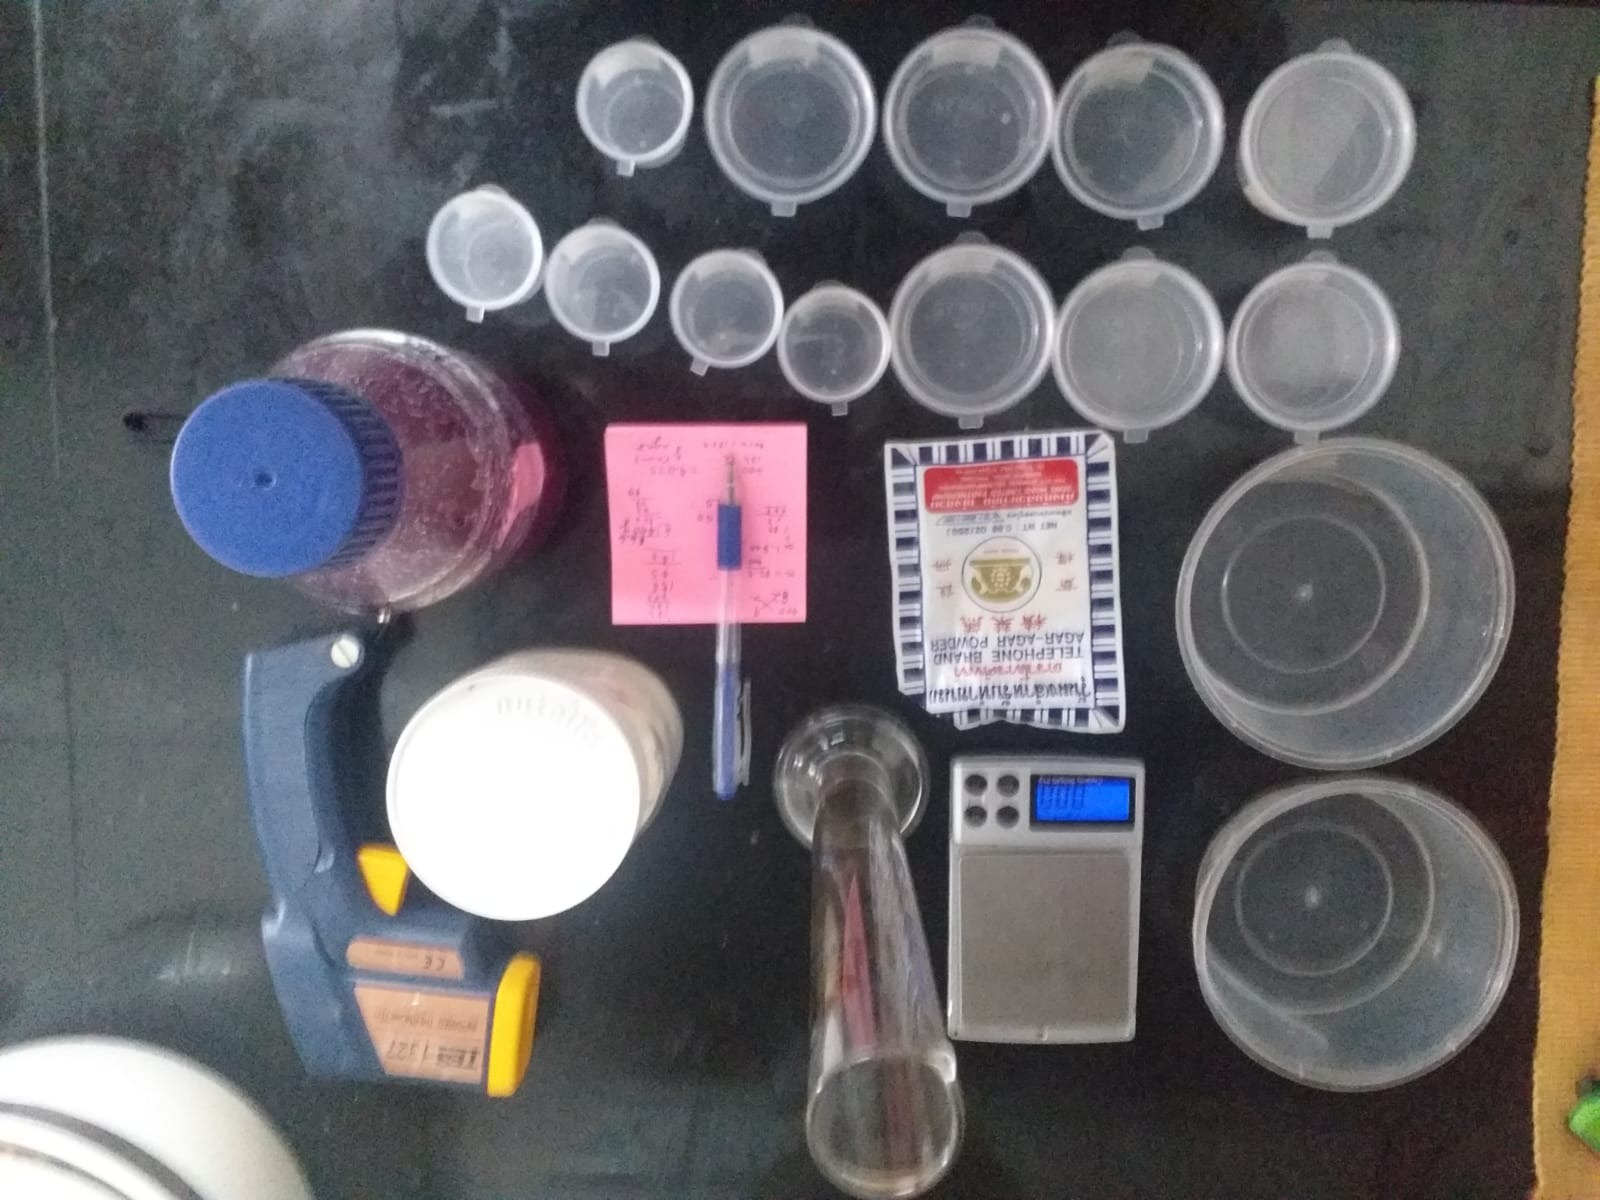
\includegraphics[width=0.5\textwidth]{Project Proposal/Photos/equipment.png}
\caption{Some necessary equipment for live culture work (preparing agar plates). PP5 grade plastic cups are used in place of petri dishes. A temperature gun is used to measure the agar temperature prior to pouring plates.}
\end{figure}

\begin{figure}[!htb]
\centering
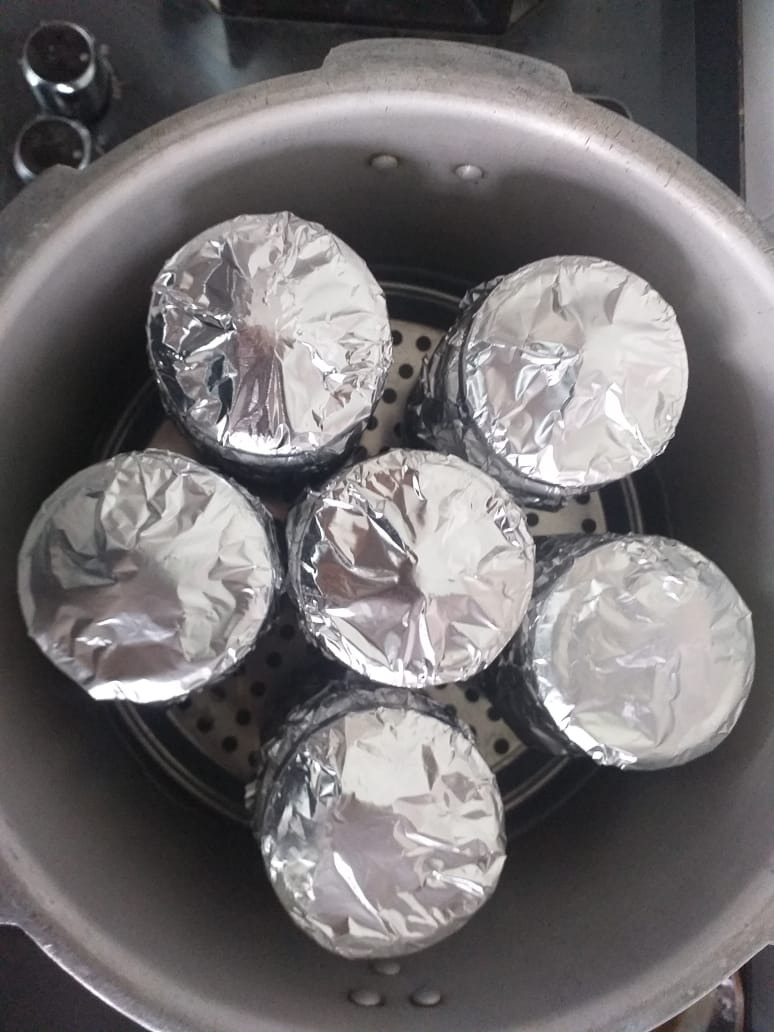
\includegraphics[width=0.35\textwidth]{Project Proposal/Photos/autoclave.png}
\caption{Jars of agar getting ready to be autoclaved for sterility in a pressure cooker (15 psi for 20 minutes). Autoclaving ensures no contaminants can grow on the agar surface.}
\end{figure}

\begin{figure}[!htb]
\centering
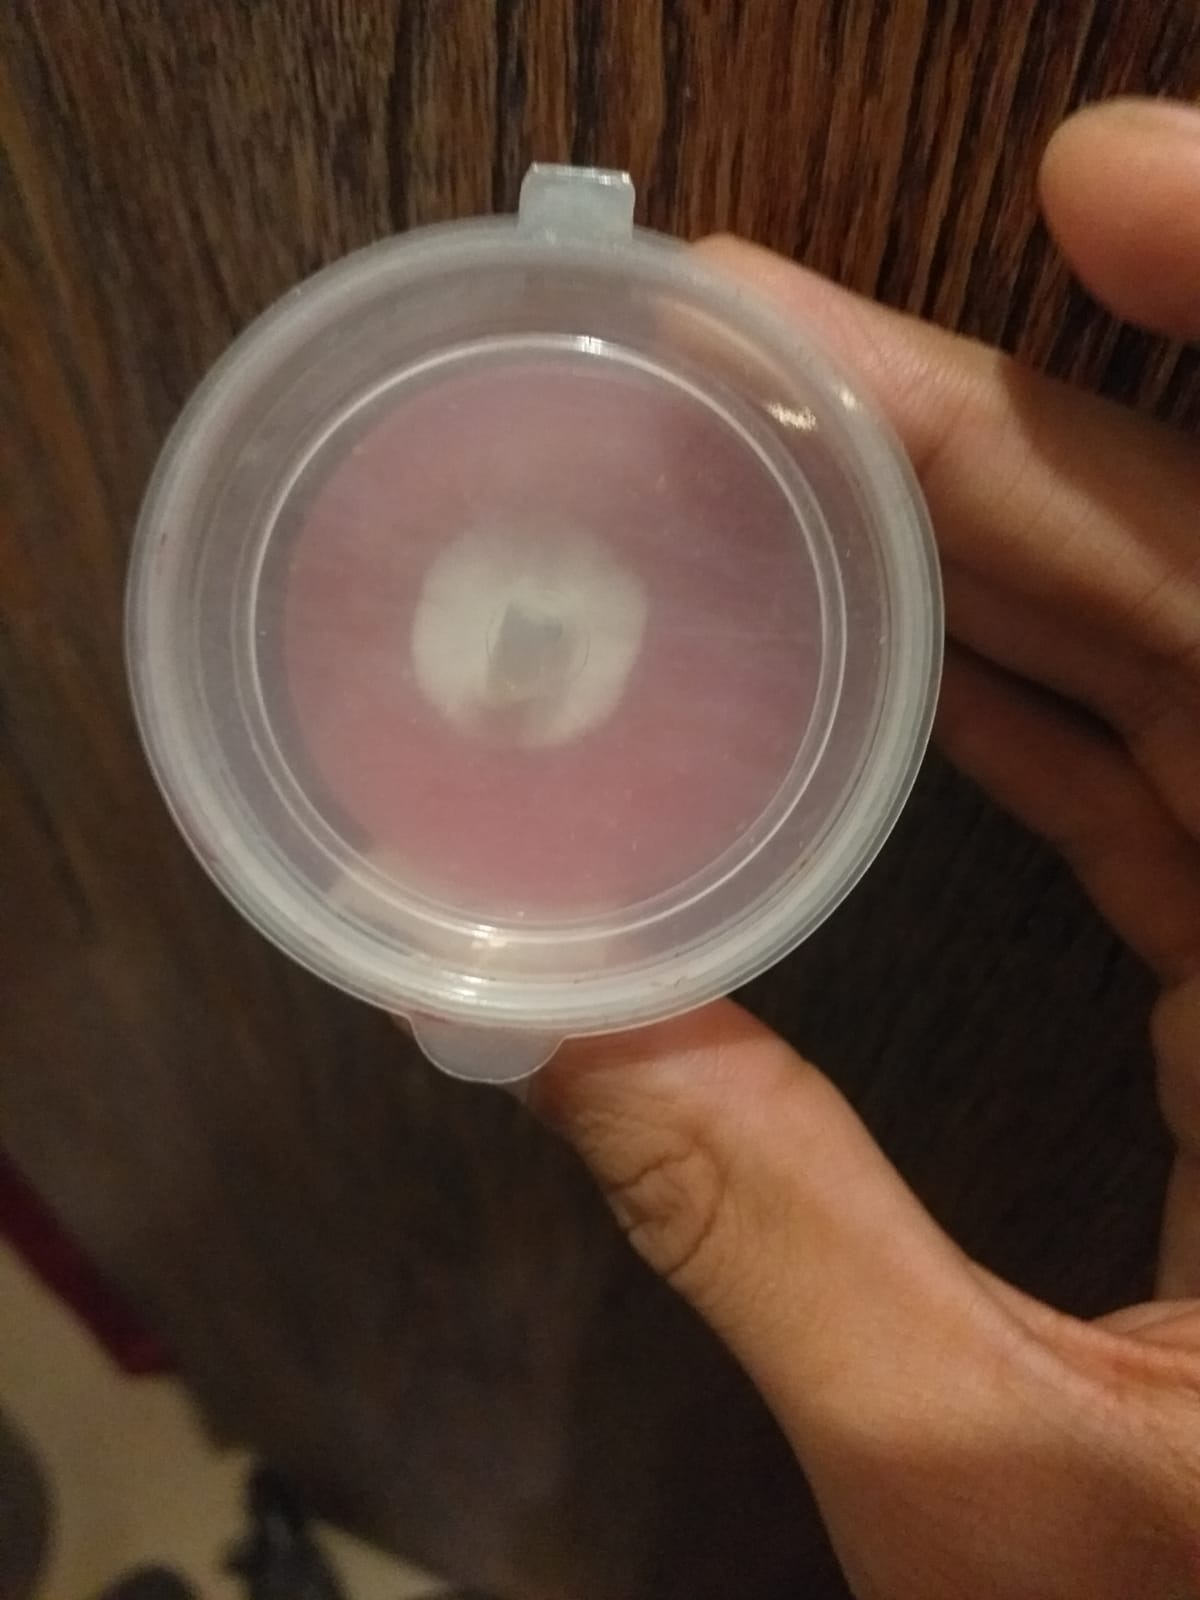
\includegraphics[width=0.4\textwidth]{Project Proposal/Photos/overhead.png}
\caption{An agar plate of wild mushroom mycelium (species unknown) cloned on 4\% brown rice flour agar.}
\end{figure}

\begin{figure}[!htb]
\centering
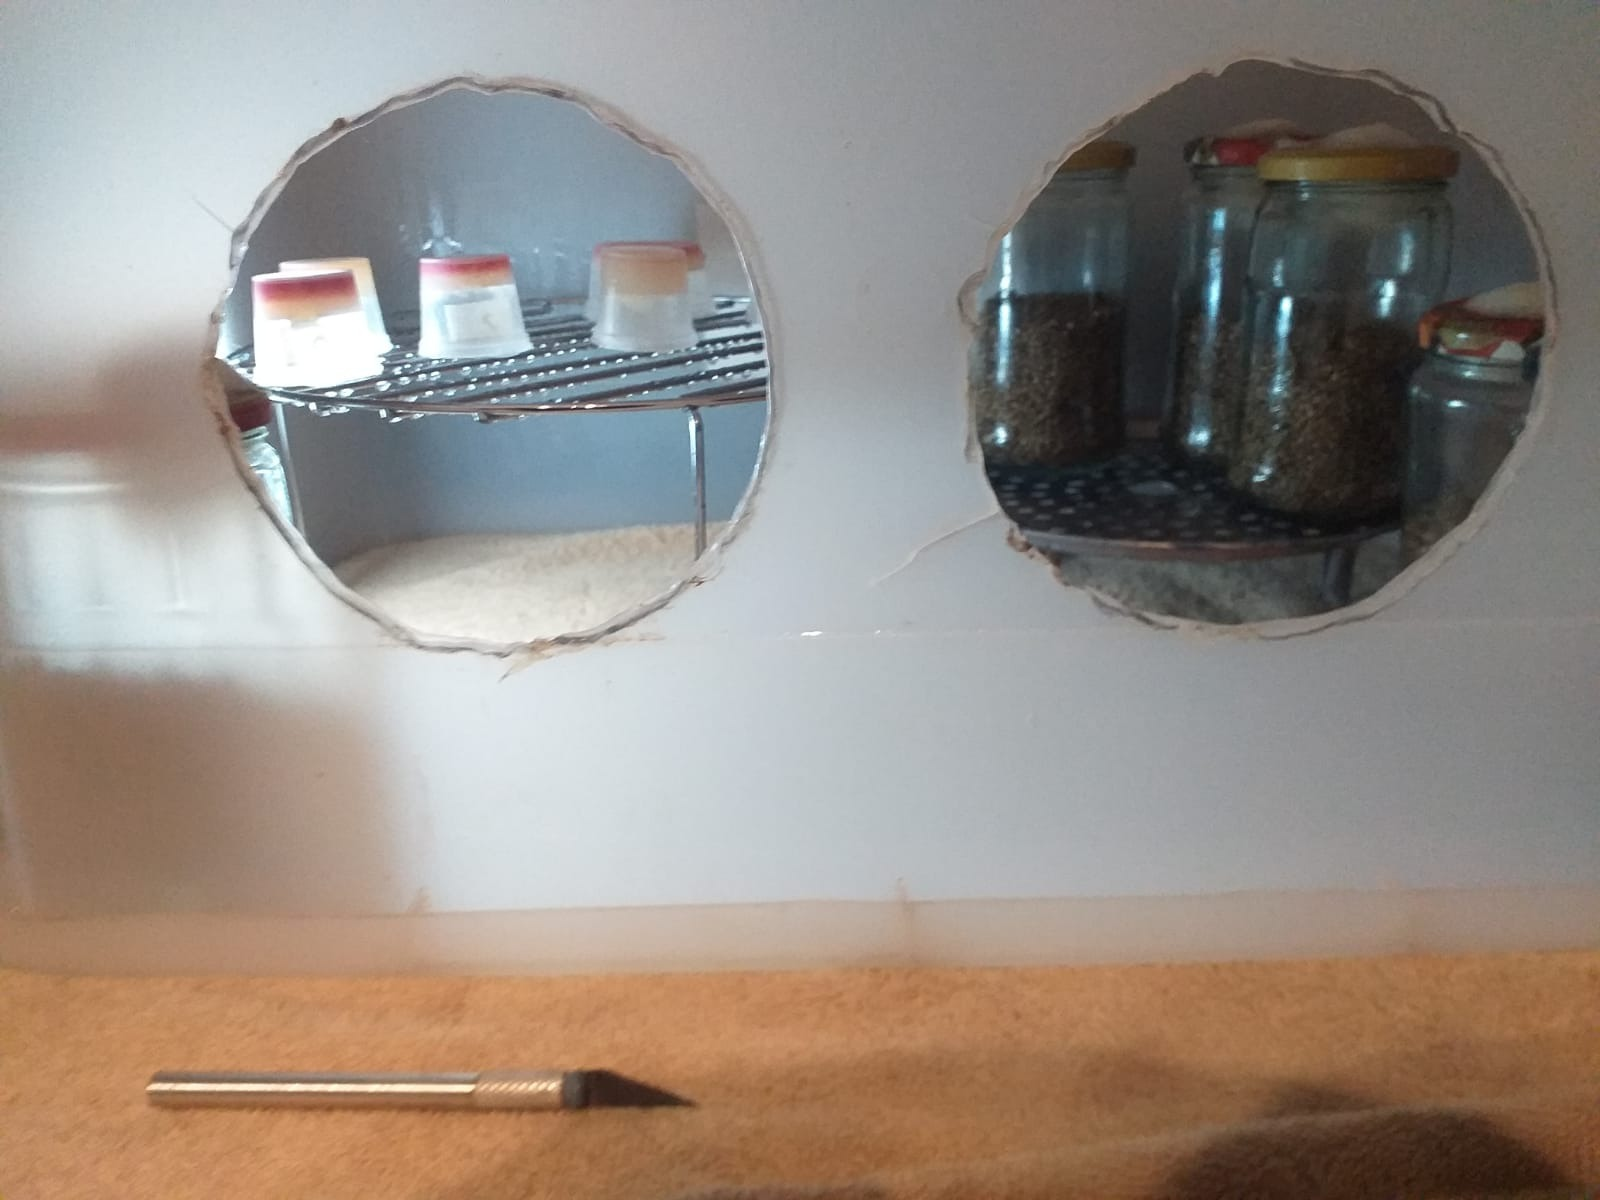
\includegraphics[width=0.5\textwidth]{Project Proposal/Photos/window.png}
\caption{A Still Air Box (SAB) for working with mycelium cultures. Agar plates placed upside down can be seen inside the SAB. A scalpel for taking agar transfers can also be seen placed outside the SAB.}
\end{figure}

\begin{figure}[!htb]
\centering
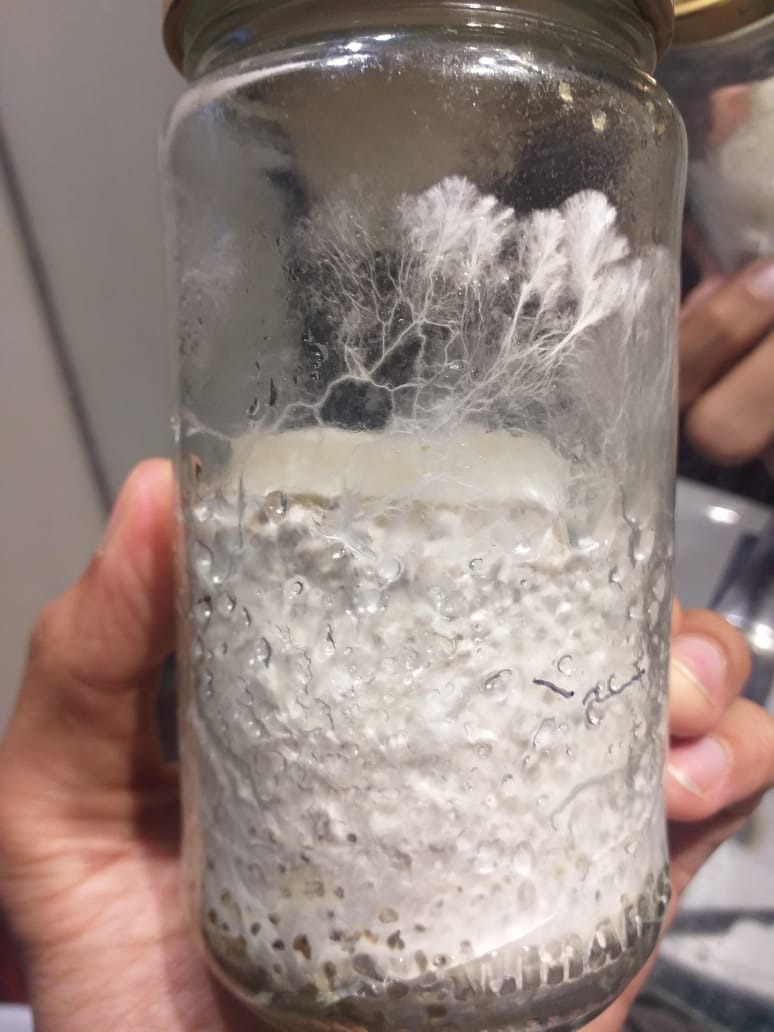
\includegraphics[width=0.4\textwidth]{Project Proposal/Photos/jar.png}
\caption{Mycelium colonizing a jar of grain. To avoid the bacteria present at the bottom the mycelium branches out in a tube-like network path at the top.}
\end{figure}

\begin{figure}[!htb]
\centering
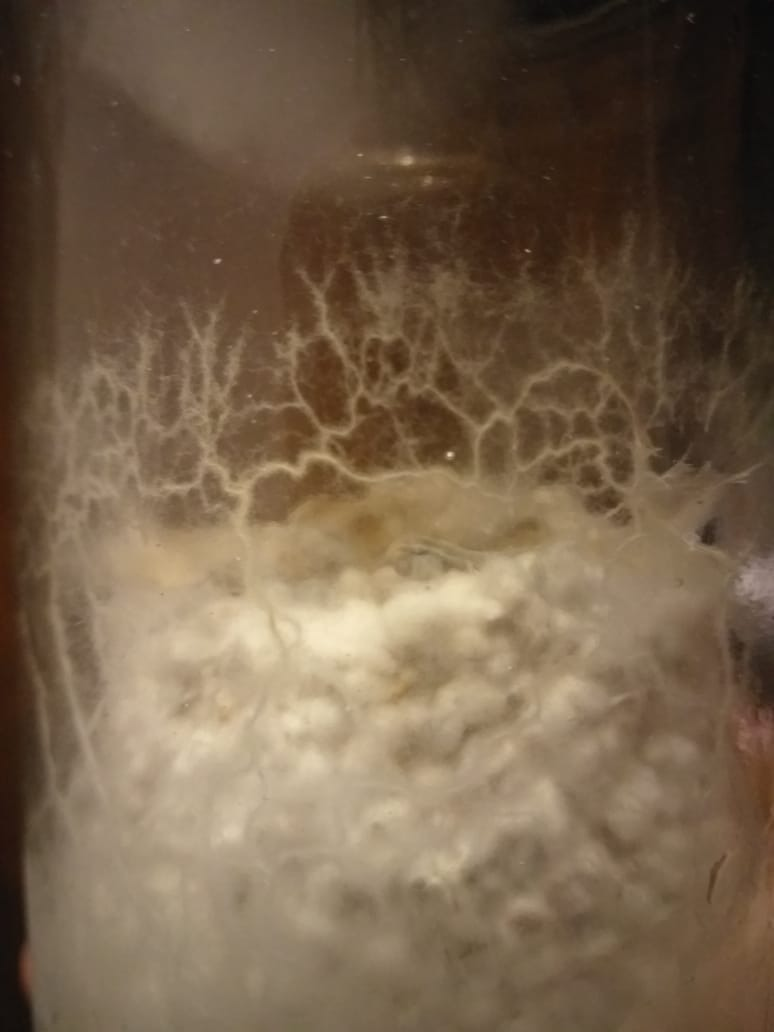
\includegraphics[width=0.4\textwidth]{Project Proposal/Photos/jar2.png}
\caption{A closeup of a mycelium network. The network is self-similar and has fractal dimension. The tubular structure shows some similarities to the organization of slime mould networks. \cite{doi:10.1098/rsfs.2018.0029}}
\end{figure}

\begin{figure}[!htb]
\centering
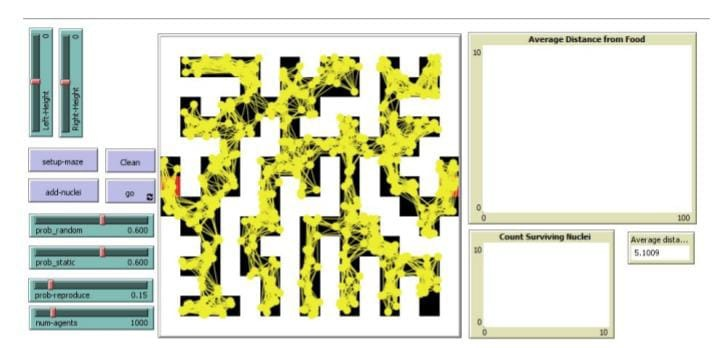
\includegraphics[width=0.9\textwidth]{Project Proposal/Photos/sim_start.png}
\caption{Starting State of Maze solving simulation (agent-based modelling in Netlogo).}
\end{figure}

\begin{figure}[!htb]
\centering
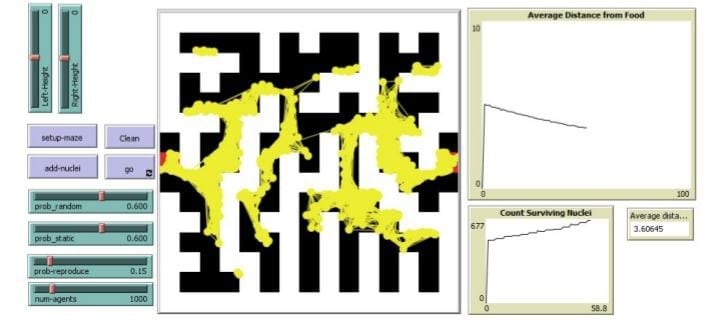
\includegraphics[width=0.9\textwidth]{Project Proposal/Photos/sim_end.png}
\caption{Final State of Maze solving simulation.}
\end{figure}

\end{document}
